
\newcommand{\tikzVec}[4]{\node[vector, rotate=#4, node distance=2cm, #1] (#2) {\rotatebox{-#4}{#3}}}
\newcommand{\vertVec}[3]{\tikzVec{#1}{#2}{#3}{00}}
\newcommand{\zHeight}{1.1cm}
\newcommand{\zExtraHeight}{\zHeight/2}
\newcommand{\zNodeDist}{(\zHeight+\zExtraHeight)/2}
\newcommand{\zCurlXShift}{0.45cm}
\newcommand{\zAmplitude}{0.4cm}
\newcommand{\Pcolor}{black!60!blue}
\newcommand{\Ncolor}{black!60!red}

\begin{tikzpicture}[
    vector/.style = {%
      draw,
      rectangle,
      drop shadow,
      fill=white,
      minimum width=0.58cm,
      minimum height=2.1cm,
      font={\scriptsize},
    },
    ae trapezoid/.style = {%
      draw,
      trapezium,
      drop shadow,
      fill=white,
      trapezium angle=75,
      minimum width=1.8cm,
      minimum height=1cm,
      thick,
    },
    net line/.style = {%
      thick,
      -latex,
    },
    enc fill/.style={
      fill=orange!10,
    },
    enc fill on/.style={alt=#1{enc fill}{}},
    latent fill/.style={
      fill=yellow!10,
    },
    latent fill on/.style={alt=#1{latent fill}{}},
    pos dec fill/.style={
      fill=blue!10,
    },
    pos dec fill on/.style={alt=#1{pos dec fill}{}},
    neg dec fill/.style={
      fill=red!10,
    },
    neg dec fill on/.style={alt=#1{neg dec fill}{}},
  ]

  \vertVec{}{xi}{$\xBase$};
  \node[ae trapezoid, right of=xi, node distance=2.4cm, rotate=-90, enc fill on=<2-2>] (enc) {\rotatebox{90}{$\fPUenc(\cdot;\theta_{e})$}};
  \draw[net line] (xi) -- (enc);

  \coordinate[right of=enc, node distance=2.5cm] (zMid);
  \vertVec{above of=zMid, minimum height=\zExtraHeight, node distance=\zNodeDist, latent fill on=<3-3>}{zP}{$\zP$};
  \vertVec{above of=zMid, node distance=0cm, minimum height=\zHeight, latent fill on=<3-3>}{zS}{$\zS$};
  \vertVec{below of=zMid, minimum height=\zExtraHeight, node distance=\zNodeDist, latent fill on=<3-3>}{zN}{$\zN$};
  \draw[net line] (enc) -- (zS);

  \coordinate[above right=0cm and \zCurlXShift of zP.north] (zpCurlTop);
  \coordinate[above right=0cm and \zCurlXShift of zS.south] (zpCurlBot);
  \draw[decoration={brace,mirror,amplitude=\zAmplitude},decorate,thick,color=\Pcolor] (zpCurlBot) -- node[right=0.35*\zAmplitude] (zPout) {} (zpCurlTop);

  \coordinate[above right=0cm and \zCurlXShift of zN.south] (znCurlBot);
  \coordinate[above right=0cm and \zCurlXShift of zS.north] (znCurlTop);
  \draw[decoration={brace,mirror,amplitude=\zAmplitude},decorate,thick,color=\Ncolor] (znCurlBot) -- node[right=0.35*\zAmplitude] (zNout) {} (znCurlTop);

  \coordinate[right of=zMid, node distance=3.2cm] (decMid);
  \node[ae trapezoid, above of=decMid, node distance=1.5cm, rotate=90, pos dec fill on=<4-4>] (decP) {\rotatebox{-90}{$\fPUp(\cdot;\theta_{p})$}};
  \vertVec{right of=decP}{xHatP}{$\xHatP$};
  \draw[net line] (decP) -- (xHatP);

  \node[ae trapezoid, below of=decMid, node distance=1.5cm, rotate=90, neg dec fill on=<5-5>] (decN) {\rotatebox{-90}{$\fPUn(\cdot;\theta_{n})$}};
  \vertVec{right of=decN}{xHatN}{$\xHatN$};
  \draw[net line] (decN) -- (xHatN);

  \newcommand{\zOutNetLength}{0.7cm}
  \coordinate[right of=zPout, node distance=\zOutNetLength] (zpOutShift);
  \draw[net line,color=\Pcolor] (zPout) -- (zpOutShift) |- (decP);

  \coordinate[right of=zNout, node distance=\zOutNetLength] (znOutShift);
  \draw[net line,color=\Ncolor] (zNout) -- (znOutShift) |- (decN);

  \onslide<6->{
    \node[left of=xi, scale=0.7, node distance=0.8in,draw] (CatIn) {
\includegraphics[width=.25\textwidth]{tikz/img/funny_cat.jpg}};
  }
  \onslide<7->{
    \node[right of=xHatP, scale=0.7, node distance=0.8in,draw] (CatOut) {
\includegraphics[width=.25\textwidth]{tikz/img/funny_cat.jpg}};
  }
  \onslide<8->{
    \node[right of=xHatN, scale=0.6, node distance=0.8in,draw] (DogOut) {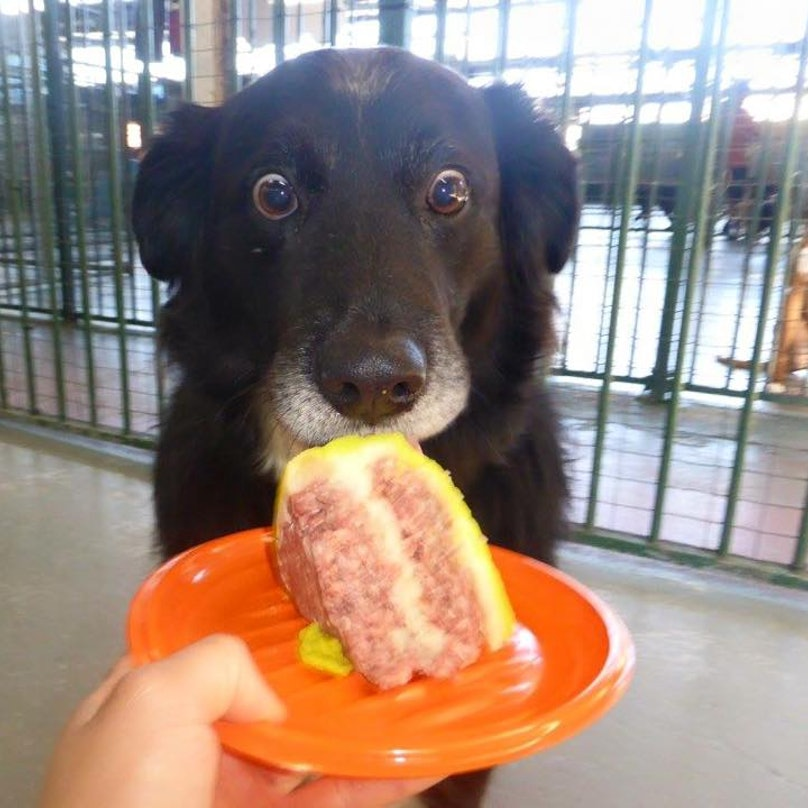
\includegraphics[width=.25\textwidth]{tikz/img/dog_face.jpg}};
  }
\end{tikzpicture}
